\documentclass{amsart}
%\usepackage{amssymb, amsmath, amsthm}
\usepackage[margin=1in]{geometry}
\usepackage{verbatim}
\usepackage{graphicx}
\usepackage{hyperref} % \url \href
\usepackage{docmute}

\newcommand{\pfrac}[2]{\frac{\partial #1}{\partial #2}}
\newcommand{\setM}{\mathcal{M}}
\newcommand{\bfx}{\mathbf{x}}
\newcommand{\bft}{\mathbf{t}}

\newtheorem*{theorem}{Theorem}
\newtheorem*{lemma}{Lemma}

\theoremstyle{remark}
\newtheorem*{remark}{remark}
\theoremstyle{remark}
\newtheorem*{example}{example}

\theoremstyle{definition}
\newtheorem*{definition}{Definition}

\DeclareMathOperator{\Aut}{Aut}
\DeclareMathOperator{\Image}{Im}
\DeclareMathOperator{\AO}{AO}
\DeclareMathOperator{\E}{E}
\DeclareMathOperator{\Sym}{Sym}
\DeclareMathOperator{\GL}{GL}
\DeclareMathOperator{\Hom}{Hom}
\DeclareMathOperator{\Tr}{trace}
\DeclareMathOperator{\Bij}{Bij}
\DeclareMathOperator{\Orb}{Orb}

% the highest level is part
% in each part, different section give different topics that are lossly connected
% subsection* should be used for giving subsequent definitions that are less important
\begin{document}


\part{Group Theory}

\section*{Mapping}
In this note, mapping and function are used interchangably. 
% https://en.wikipedia.org/wiki/Bijection,_injection_and_surjection
\subsection*{Injective}
A mapping is called injective (one-to-one) if each element of the codomain is mapped by 
at most one element of the domain (arguments, input). 
For all $x,x' in X$, $f(x)=f(x')$ only if $x=x'$.

\subsection*{Surjective}
A function is surjective (onto), if each element of the codomain is mapped to by at least one element of 
the domain. That is, the image of of the domain equals the codomain. 
For all $y\in Y$, there exist an $x\in X$ so that $y=f(x)$.

\subsection*{Bijection}
If the function is both injective and bijective, than it is called bijective. Bijective is also called invertible.

\begin{figure}[h!]
    \centering
    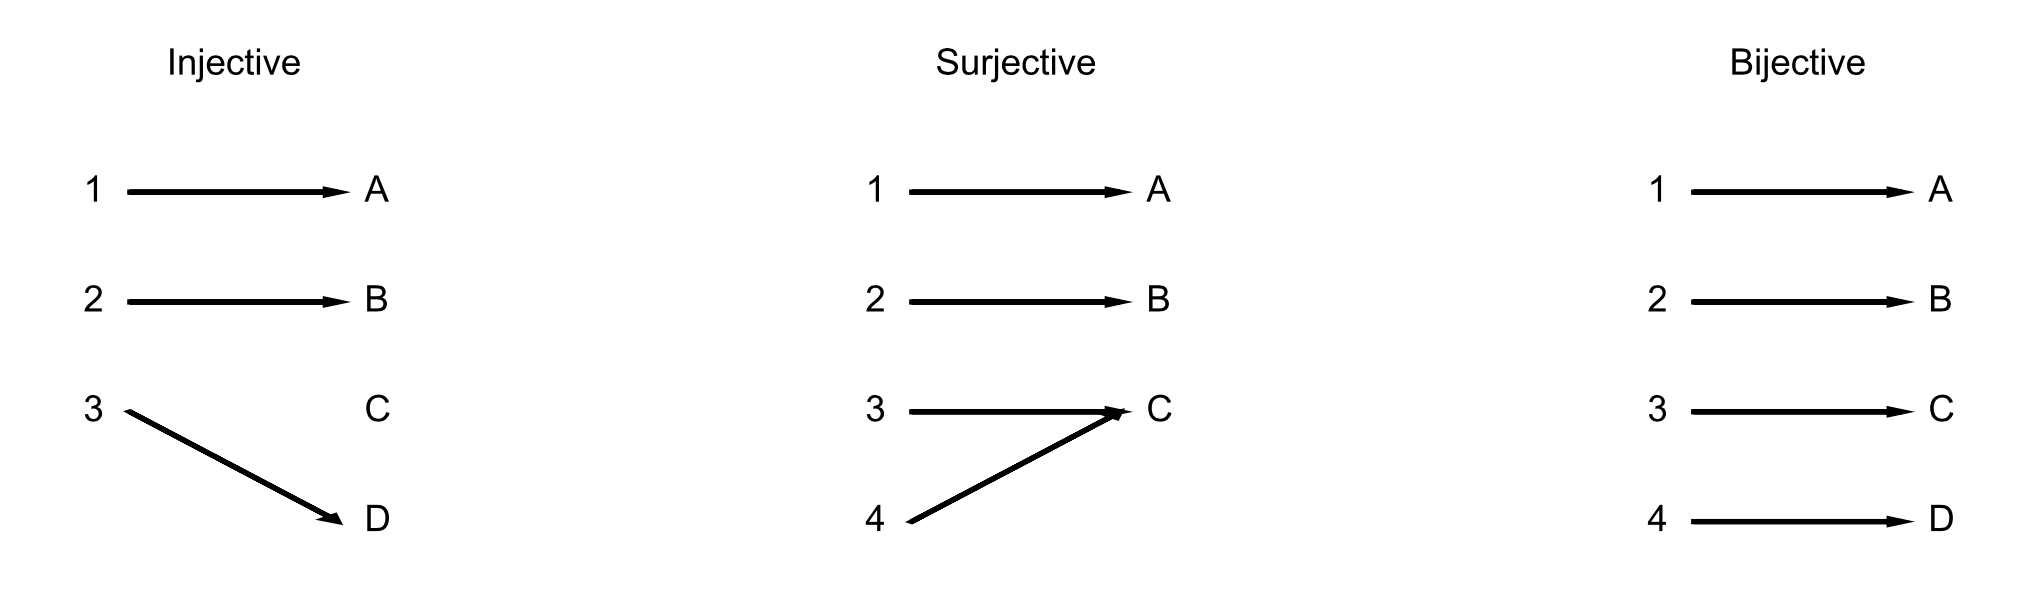
\includegraphics[width = 5in]{figures/mapping.png}
\end{figure}

\vspace{10pt}
\section*{Definition of Group}
\begin{definition}[Group]
    A group is a set plus an operation, that map an ordered pair of group element $(g,h)$ of $G$ into another element $g\cdot h \in G$, satisfying
    the following properties:
    \begin{enumerate}
        \item operation is associative: $g\cdot (h \cdot k) = (g\cdot h) \cdot k$ for $g,h,k \in G$;
        \item $G$ contain an identity element $e$, that satisfies $g\cdot e = e\cdot g = g$ for all $g \in G$ and 
        \item Each element of $G$ has an inverse, denoted by $g^{-1}$.
    \end{enumerate}  
\end{definition}

\subsection*{Order of the group}
    Order of the group $G$, or the cardinality of the group, is the number of elements in the set $G$, denoted by $|G|$


\vspace{10pt}
\section*{Two important group}

\subsection*{Linear transformation group}
Denoting $V$ as a vector space on field $F$, we write $\text{GL}(V)$ (general linear) as the set of all \emph{invertible linear transformation} in $V$. 
Since $g\in GL(V)$ is invertible and the product of two invertible linear transformation is again an invertible transformation, $GL(V)$ 
form a group. The group elements map a vector $v\in V$ to another vector $v' \in V$. Invertible means that the determinant of the 
matrices are non-zero.

\subsection*{Permutation group}
Denoting a set by $X$. All the bijections of $X$ to itself form a group, which we denote $\Sym(X)$. 

\vspace{10pt}

For a set $X$ with $n$ elements $|X| = n$, the total number of possible bijection (permutation) is $n!$. Therefore $|\Sym(X)| = n!$.
Since we care about bijections $X\to X$, not the set $X$ itself, Therefore, for two sets with the same number of elements,
$|X| = |Y|$, their permutation group is the same: $\Sym(X) = \Sym(Y)$ and we simply denote it as $\Sym(n)$ or $S_n$.

\subsubsection*{Two line notation of permutation}
We denote a permutation by $\pi\colon \{1,2,\dots,n\} \to \{ \cdots \}$. For example:
\[
    \pi = \left(  
    \begin{matrix} 
    1&2&3&4&5\\
    5&4&1&2&3
    \end{matrix}
    \right) \in S_5
\]
gives a permutation $\{1,2,3,4,5\} \to \{ 5,4,1,2,3 \}$. Such notation is called 'two-line notation'
We should note that the numbers are to be interpreted as indices of the objects in the set.

\subsubsection*{Matrix notation}
In matrix form, we have:
\begin{equation*}
    \left( \begin{matrix} 5 \\ 4 \\ 1 \\ 2\\ 3 \end{matrix} \right)
    = \left( \begin{matrix} 
        0 & 0 & 0 & 0 & 1 \\
        0 & 0 & 0 & 1 & 0 \\
        1 & 0 & 0 & 0 & 0 \\
        0 & 1 & 0 & 0 & 0 \\
        0 & 0 & 1 & 0 & 0 
    \end{matrix} \right) 
    \left( \begin{matrix} 1 \\ 2 \\ 3 \\ 4 \\ 5 \end{matrix} \right)
\end{equation*}
We call the matrix of permutation $A_{\pi}$. 
With the matrix notation, we can define the sign of a permutation:
\[\text{sign}\pi = \det A_{\pi}\]

\subsubsection*{Cyclic notation}
For the example permutation $\{1,2,3,4,5\} \to \{ 5,4,1,2,3 \}$, we can simply write
$\pi = (153)(24)$
The interpretion of cyclic notation is as follows:
\begin{itemize}
    \item a cyclic is a permutation of a subset without affecting other elements,
    \item fixed point can be omitted,
    \item $(153)$ is read as $1\to 5, 5\to 3, 3\to 1$. $1\to5$ reads 'object in position 1 become object in position 5'.
\end{itemize}
We can generate the two-line notation from the cyclic notation as follows:
\begin{equation*}
    \begin{matrix}
                & 1 & 2 & 3 & 4 & 5 \\
        1 \to 5 \quad & 5 &   &   &   &   \\
        5 \to 3 \quad &   &   &   &   & 3 \\
        3 \to 1 \quad &   &   & 1 &   &   \\
        2 \to 4 \quad &   & 4 &   &   &   \\
        4 \to 2 \quad &   &   &   & 2 &   \\
                & 5 & 4 & 1 & 2 & 3
    \end{matrix}
\end{equation*}

The following arrow form of permutation is also convenient to keep track of the operation, especially for successive 
application of permutations. Note that the arrow $5\to1$ reads 'the object in position 5 is moved to position 1'.
\begin{figure*}[!h]
    \centering
    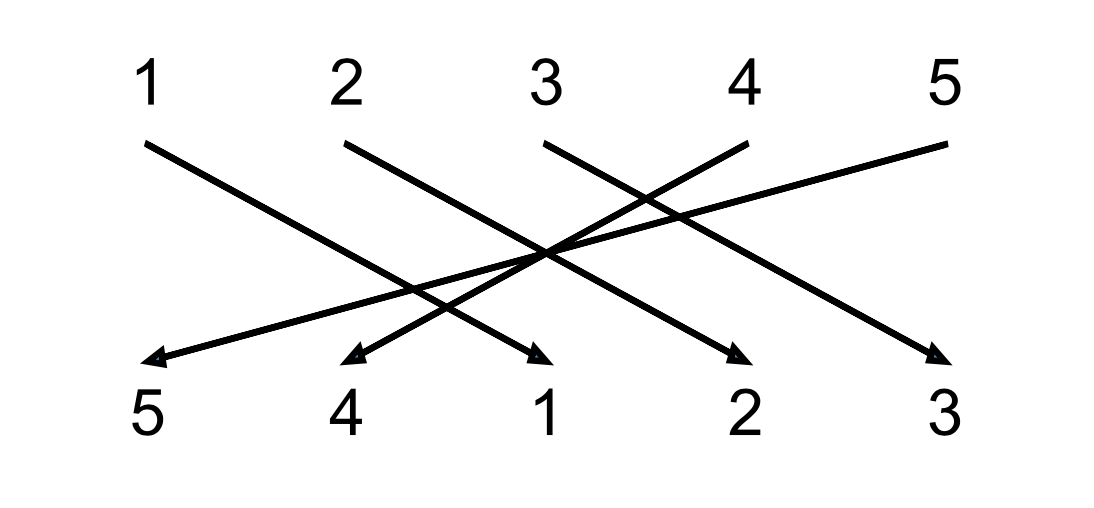
\includegraphics[width=2in]{figures/permutation_arrow.png}
\end{figure*}

\vspace{10pt}
\section*{Multiplication Table}
\subsection*{Multiplication Table}
Multiplication table shows how a group element are obtained by the product of two group element. We illustrate the multiplication 
table using the group $S_3$.
Using cyclic notation, we can write $S_3 = \{ e, (1,2), (2,3), (1,3), (1,2,3), (3,2,1) \}$. We have $|S_3| = 6$. The group table of $S_3$ can be calculated 
and tabulated to be:
\begin{table}[h]
    \centering
    \caption{Multiplication table of $S_3$}
    \begin{tabular}{|c|ccc|ccc|}
        \hline
                & e     & (123) & (321) & (12)  & (13)  & (23)  \\ \hline
           e    & e     & (123) & (321) & (12)  & (13)  & (23)  \\ 
          (123) & (123) & (321) & e     & (13)  & (23)  & (12)  \\
          (321) & (321) & e     & (123) & (23)  & (12)  & (13)  \\ \hline
          (12)  & (12)  & (23)  & (13)  &     e & (321) & (123) \\
          (13)  & (13)  & (12)  & (23)  & (123) & e     & (321) \\
          (23)  & (23)  & (13)  & (12)  & (321) & (123) & e     \\ \hline
    \end{tabular}
    \label{T:s3}
\end{table}

\begin{remark}
    We can varify for $S_3$, two elements $(12)$ and $(123)$ generate the whole group. 
    This result is also true for permutation group of higher order: For $S_n$, two elements
    $(12)$ and $(123\dots n)$ generate the whole group.
    (Not arbitrary two elements can generate the whole group: consider for $S_4$, two elements $(12)$ and $(23)$ will
    only permute index 1,2,3 but will not touch the fourth item. Of course, this two element generator set is not 
    the only generator set possible.)
\end{remark}

\vspace{10pt}
\section*{Subgroups}

\begin{definition}[Subgroup]
    Definition: $H$ is a non empty subset of $G$ and $H$ is a group, then $H$ is a subgroup of $G$
\end{definition}
For group $S_3$, we can find four non-trival subgroups: $\{e, (12)\}$, $\{e, (13)\}$, $\{e, (23)\}$ and $\{e, (123), (321)\}$

\begin{theorem}
    The intersections of subgroups of $G$ is also a subgroup of $G$.
\end{theorem}
\begin{proof}
    Suppose $H$ and $L$ are subgroups of $G$. $M$ is the intersections between $H$ and $L$, then:
    \begin{enumerate}
        \item identity $e \in M$;
        \item if $h_1, h_2 \in H$ and $h_1 \cdot h_2 = e$, If $h_1\in L$, then inevitably $h_2 \in L$, therefore the intersections of $H$ and $L$ is closed under inverse;
        \item similarly, if $h_1, h_2 \in H$ and $h_1, h_2 \in L$, then $h_1\cdot h_2$ belong to both $H$ and $L$ are therefore in the intersections. $M$ is closed under group operation.
    \end{enumerate}
\end{proof}

\begin{definition}[Generator]
    For a set $S$, the intersections of all subgroups contain $S$ is a subgroup. 
    This intersections is denoted by $\langle S\rangle$ and we say that it is generated by $S$. 
\end{definition}


For a group element $g$, we write that group that is generated by $g$ as $\langle g \rangle$, the order of $\langle g \rangle$ is also called the order of $g$. 

\subsection*{Cyclic group}
A group is called a cyclic group if it is generated by a single element, i.e., $G = \langle g \rangle$.

\begin{lemma}
    if a group $G$ is finite, we must have $g^n = e$ for $g \in G$. Since any $g^a$ is a number in $G$
\end{lemma}

\vspace{10pt}
\section*{Multiplication of group} 

\subsection*{Group multiplication}
For $S$ and $T$, both subset of group $G$, we define their product:
\begin{equation*}
    ST = \{st\mid s\in S, t \in T\}
\end{equation*}
and $sT \equiv \{s\}T $ and $Ts \equiv T\{s\} $ for $s \in S$.

\vspace{10pt}

\begin{definition}[Left cosets]
    For $H$ a subgroup of $G$ and $g \in G$, $gH$ is called a left coset. $Hg$ is called a right coset. 
    The set $\{gH \mid g \in G, H\ \text{is subgroup of}\ G\}$ is written as $G/H$
\end{definition}

For example, for $S_3$ and its subgroup $H = \{e,(123),(132)\}$, 
Using the multiplication table \ref{T:s3}, we can find that
applying element $g \in \{(12), (23), (13)\}$ on $H$
give the set $\{(12), (23), (13)\}$. Therefore, the left cosets of $H$ is:
\[
    \left\{\, \{e,(123),(132)\}, \{(12), (23), (13)\}\, \right\}    
\]

\begin{theorem}
    The left cosets of the subgroup $H$ of $G$ partition $G$
\end{theorem}
\begin{proof}
    This is equivalent to say that $gH$ is either $H$ itself, or share no comment elements with $H$.
    if $g\in H$, then $gH = H$. On the other hand, 
    if $g\notin H$ but $gh \in H$ for an element $h\in H$, then, by the requirement of group $h^{-1}\in H$. $ghh^{-1} = g \in H$ which conflict with the assumption.
    Therefore, we $gH$ cannot share element with $H$: $|gH| = |H|$, so that left cosets of a subgroup partition the group.
\end{proof}
As a result, the whole group can be written as:
\[
    G = H + g_1 H + g_2 H + \dots + g_n H    
\]
\begin{theorem}[Lagrange's theorem]
    For a finite group $G$ and $H$ is a subgroup of $G$, $|H|$ can divide $G$.
\end{theorem}
\subsection*{Index of $H$ in $G$}
    The number of left cosets of a subgroup $H$ is called the index of $H$ in $G$, denoted as $[G:H]$.
\begin{remark}
    If $G$ is a finite group and $g\in G$. Then the order of $\langle g\rangle$ divide $|G|$. This is because 
    $\langle g\rangle$ is a subgroup of G.
\end{remark}

\vspace{10pt}
\section*{Mapping}

\begin{definition}[Homomorphism]
    We define a mapping $\Phi\colon G \to H$ from group $G$ to $H$. If
    \[
        \Phi(g_1 g_2) = \Phi(g_1) \Phi(g_2)    
    \] 
    is satisfied for all $g_1, g_2 \in G$, then we call $\Phi$ a homomorphism
\end{definition}

\subsection*{Isomorphism}
    If the mapping $\Phi$ is a bijection, then we call $\Phi$ an isomorphism. If $G$ and $H$ are related by 
    an isomorphism, we write $G\cong H$

\begin{remark}
    Isomorphic groups have the same group multiplication table, apart from the names or symbols and, if necessary, after 
    rearranging rows and columns. 
    With the aid of isomorphism, all groups can be subdivided into \emph{isomorphism classes} of isomorphic groups. 
    Such a class is known as an \emph{abstract group}, each group within the isomorphism class are called 
    \emph{realization of the abstract group}
\end{remark}

\subsection*{Automorphism}
    We call the mapping $\Phi\colon G \to G$ (from $G$ onto itself) an automorphism. We write the set of all automorphism by $\Aut(G)$ 
\begin{remark}
Automorphism are bijections. For example, $\Phi\colon G \to gG$ is an automorphism, 
this is shown in the rearrangement theorem. 
\end{remark}

\vspace{10pt}

\begin{theorem}[Rearrangement theorem]
    for group $G$ and a group element $g'\in G$, the set 
    \[\{g'g \mid g \in G\}\]
    contain each group element once and only once.
\end{theorem}
\begin{proof}
    It is equivalent to say that if $g_1 \neq g_2$, then $g'g_1 \neq g'g_2$. all group element in $G$ are mapped 
    to another distinct elements in $G$ (rearrangement).

    If $g'g_1 = g'g_2$ but $g_1 \neq g_2$, then 
    \[ g'^{-1}g'g_1 = g'^{-1}g'g_2 \] which apperant conflict with the assumption
\end{proof}

\vspace{10pt}

\begin{definition}
    [Kernel] For a homomorphism $\Phi\colon G \to H$, we define the kernel $\ker\Phi = \{g\in G\mid \Phi(g) = e_h \}$, i.\,e.\,,
    kernel of $\Phi$ is the elements in $G$ that are mapped to identity of group $H$. $\ker\Phi \subset G$
\end{definition}

\begin{definition}
    [Image] For homomorphism $\Phi\colon G \to H$, we define the image $\Image\Phi = \{ \Phi(g) \mid g \in G \}$, i.\,e.\,,
    the elements in $H$ that are obtained from the mapping. $\Image\Phi \subset H$
\end{definition}

\begin{lemma}
    $\ker\Phi$ is a subgroup of $G$
\end{lemma}
\begin{lemma}
    $\Image\Phi$ is a subgroup of $H$
\end{lemma}

\vspace{10pt}

\begin{theorem}
    Homomorphism $\Phi\colon G\to H$ is injective if and only if $\ker \Phi = e$
\end{theorem}
\begin{proof}
    If $\Phi$ is injective, then we require $\ker \Phi = e_g$; 

    If $\ker \Phi = e_g$. Suppose $\Phi(a) = h$ and $\Phi(b) = h$. If in group $G$, we have $ax = b$, with $x\in G$, 
    Then we have:
    \[  
        \Phi(b) = \Phi(a)\Phi(x)    
    \]
    This implies that $\Phi(x)=e_h$ and $x = e_g$. Therefore, $a = b$: if $\ker \Phi = e_g$ then we cannot have
    two different elements in $G$ that are mapped to the same element in $H$.
\end{proof}

\vspace{10pt}
\section*{Conjugation of group elements}

\begin{definition}
    [Conjugate classes]
    Two group elements $a$ and $b\in G$ are called conjugate if there is another element $g$, so that:
    \[g^{-1}ag = b\]
    The elements of $g$ can then be collected into classes. $C_k$, each is made of conjugate elements. 
\end{definition}
\begin{remark}
    if $a$ is conjugate to $b$ and $b$ is conjugate to $c$, then $a$ is conjugate to $c$:
    \[ c = h^{-1}bh = h^{-1}g^{-1}agh = (gh)^{-1}a gh \]
\end{remark}
Conjugate partition $G$ into \emph{equivalent classes}. $C_a = \{g^{-1}ag\mid g\in G\}$ is called conjugacy class 
from $a$. 
As an example, for group $S_3$, with the help of multiplication table, we have the following conjugate classes:
\begin{align*}
    g^{-1}eg &= e  & (12)(123)(12) &= (321) & (12)(12)(12) = (12) \\
    &&  (13)(123)(13) &= (321) & (13)(12)(13) = (23) \\
    &&  (23)(123)(23) &= (123) & (23)(12)(123) = (13) \\
    &&  (321)(123)(123) &= (123) & (321)(12)(123) = (13) \\
    &&  (123)(123)(321) &= (123) & (123)(12)(321) = (23)
\end{align*}
Therefore, the conjugate classes are $\{e\}, \{(12),(23),(13)\}, \{(123),(321)\}$. 

We have the following general results for conjugate classes:
\begin{enumerate}
    \item Each element is at least conjugate to itself: $g^{-1}gg = g$,
    \item Every element in $G$ belongs to exactly one conjugacy class,
    \item Numbers of elements in conjugacy classes are different, but they are always divisor of order of $G$,
    \item Elements in the same conjugacy class have the same order.
\end{enumerate}

\subsection*{Self-conjugate elements}
If for $g_i\in G$ and we have $g_m^{-1}g_i g_m = g_i$ for all $g_m \in G$, then $g_i$ is called \emph{self-conjugate}.
\begin{remark}
    Since $g_m^{-1}g_i g_m = g_i$ means $g_i g_m = g_m g_i$, self-conjugate condition means that $g_i$ commute with all 
    elements in the $G$. 
    It is straightforward to see that identity element is always self-conjugate. 
\end{remark}

\subsection*{Abelian group}
A group is called abelian if for all $g, h \in G$, $g\cdot h = h \cdot g$. 
Therefore, each element $g\in G$ form a conjugate classes by its own.

\vspace{10pt}
\section*{Conjugating subgroups and Quotinet group}

Previous definition of conjugating is defined on elements. For subgroups, we also have similar definitions:
\begin{definition}
    [Conjugate subgroups]
    Two subgroup $H$ and $H'$ are called conjugate subgroups in $G$ if there exist an element $g_i\in G$
    so that $H' = g_i^{-1}Hg_i$, i.e., the left coset and the right coset formed from $H$ and $g_i$ are the same. 
\end{definition}
\begin{remark}
    The set of subgroups that are conjugate to $H$ form a conjugacy class. 
    The conjugate subgroups are isomorphic and have the same order.
\end{remark}
From the multiplication table of $S_3$, we find conjugating subgroups:
\begin{equation*}
    \overbrace{\{e, (123), (321)\}}\quad \overbrace{\{e, (12)\},\{e, (13)\},\{e, (23)\}}
\end{equation*}

\begin{definition}
    [Normal subgroup]
    A subgroup is called normal (self-conjugate) if 
    \[
        gHg^{-1} = H\quad \text{for all}\ g \in G 
    \]
    Equivalently, this means that every left cosets of $H$ in $G$ is also a right coset of $H$ in $G$.
\end{definition}
We can see that the subgroup $\{e, (123), (321)\}$ of $S_3$ is a normal subgroup: it only conjugate with itself.

If $H$ is a normal subgroup, then for the set $G/H$, we can show that $(g_1 H)\cdot(g_2 H)$ is also in 
set $G/H$:
\begin{proof}
    Since $H$ is a normal subgroup, by definition: 
    \[gH = Hg = gHg^{-1}g\] so that we fine:
    \[gHg^{-1} = H\]
    Then:
    \begin{align*}
        (g_1 H)\cdot(g_2 H) &= g_1 H g_1^{-1}g_1 g_2 H = H g_1 g_2 H \\
            &= (g_1g_2)(g_1g_2)^{-1} H (g_1g_2) H \\
            &= g_1g_2 H H = g_1 g_2 H 
    \end{align*}
    since $g_1 g_2 H$ is also a left coset and belong to $G/H$, we have shown that the set $G/H$ is indeed a group with 
    operation $(g_1 H)\cdot(g_2 H)$
\end{proof}

we call the group $G/H$ \textbf{quotinet group}, or factor group.
For example, for $H = \{e,(123),(132)\}$, the set ${H, (12)H}$ is the factor group.

\begin{lemma}
    The kernel $\ker\Phi$ of $\Phi\colon G\to H$ is a normal subgroup.
\end{lemma}

\begin{lemma}
    For a group homomorphism $\Phi\colon G\to H$, the quotinet group is isomorphic to $\Image\Phi$ (bijection).
\end{lemma}

\vspace{10pt}

\begin{definition}
    [Inner Conjugation]
    We call the mapping $\Phi_g\colon G\to G$ with $\Phi_g(h) = ghg^{-1}$ a conjugation with $g$, or an \emph{inner conjugation}
\end{definition}
According to definition, $\Phi_g \in \Aut(G)$


\vspace{10pt}
\section*{Action of a group}

\begin{definition}
    [Action of a group]
    For a group $G$ and a set $\setM$, the action of $G$ on $\setM$ is a mapping 
    $\alpha\colon G\times \setM \to \setM$ satisfying:
    \begin{enumerate}
        \item $\alpha(e,m) = m$ for $m \in \setM$;
        \item $\alpha(g, \alpha(h,m)) = \alpha(gh, m)$ for $m\in \setM$ and $h,g\in G$
    \end{enumerate}
\end{definition}
where $\alpha(g,m)$ means action of a group element $g$ on a set element in $\setM$

\begin{remark}
For an action of the group $\alpha$, 
we have a group homomorphism that map the the group actions to permutations on $\setM$. 
(Recall that permutations on $\setM$ is all the bijection that map $\setM$ to itself.) 
The homomorphism $\theta\colon G \to \Bij(\setM)$ is given by:
\begin{equation*}
    g\to (m\to \alpha(g,m))
\end{equation*}
$m\to \alpha(g,m)$ being a permutation.     
\end{remark}

\begin{definition}
    [Symmetry]
    A group element $g\in G$ is called a symmetry on set $\setM$ if it leave the set invariant:
    $\setM = \{gm \mid \text{for all }\ m \in \setM\}$. 
\end{definition}

\begin{comment}
\subsection*{Group action on itself}
For a group $G$, $G$ can act on itself by conjugation: $\alpha\colon G\times G \to G$ given by
$\alpha(h,g) = hgh^{-1}$

\begin{definition}
    [Symmetry]
    For a group $G$ acting on $\setM$, $T\subset M$ is called invariant under $S \subset G$ if $ST\subset T$, 
    with $ST = {\alpha(g,m)\mid g \in G, m\in T}$. 
    The elements in $S$ are called 'symmetry'.
\end{definition}

\end{comment}
\vspace{10pt}

\begin{definition}
    [Orbit under $G$]
    For $G$ acting on $\setM$, the sets $\Orb(m) = \{gm\mid g\in G\}$ partition the set $\setM$. 
    \[\setM = \Orb(m_1) + \Orb(m_2) + \dots + \Orb(m_n)\]
    Each set $\Orb(m)$ is called the orbit of $m$ under $G$.
\end{definition}

\subsection*{Transitive}
A group action, of $G$ on $\setM$, is called transitive if it has only one orbit, i.e., 
$\setM = \{gm \mid g \in G\}$ for some choice of $m$. A group is called transitive if 
its group action is transitive. 
The set $\setM$ of a transitive group action is called \emph{homogeneous space} if the group 
is a lie group.

\subsection*{Stabilizer}
For group $G$ acting on $\setM$ and $m \in \setM$, the set 
\[G_m = \{ g\in G\mid gm = m \}\]
are called the stabilizer of $m$. $G_m \subset G$
\footnote{stabilizer $G_m$ is not necessarily a normal subgroup of $G$}

\begin{lemma}
    Stabilizer $G_m$ is only normal if $G_m$ is also the stabilizer of every orbits of $m$: 
    if $g\in G_m$ stabilize any orbit of $m$ generated by $t\in G$, 
    we have: $gtm = tm$ and thus $t^{-1}gtm = m$. So that $t^{-1}gt \in G_m$ and $G_m$ is self-conjugating. 
    % https://proofwiki.org/wiki/Stabilizer_is_Normal_iff_Stabilizer_of_Each_Element_of_Orbit
\end{lemma}

\begin{theorem}
    [Orbit-Stabilizer theorem]
    The stabilizer $G_m$ is a subgroup of $G$, therefore, $|G_m|$ divide $G$. 
    Further more, $G_m$ is a normal subgroup. It's left cosets form a quotinet group $G/G_m$. 
    The mapping $f\colon \Orb(m) \to G/G_m$ is a bijection and $|G|=|G_m||\Orb(m)|$
\end{theorem}
\begin{remark}
    We call a
    subset of $\setM$ \emph{fundamental set} if it contain exactly one element from each orbit.
\end{remark}

\vspace{10pt}
\section*{Isometry}
The distance in euclidean space is given by 
\[
    d(x,y) = \|x-y\| = \sqrt{\sum_i(x_i-y_i)^2}    
\]

\begin{definition}
    [Isometry]
    A invertible mapping $g\colon \mathbb{E}^n \to \mathbb{E}^n$ satisfying 
    \begin{equation*}
        d(g(x),g(y)) = d(x,y)
    \end{equation*}    
    is called an isometry, i.e., the transformation that keep the distance. 
    We denote them $\E(n)$
\end{definition}
\begin{remark}
    See definition below, isometry is an affine transformation, can be written as AO(3).
    % http://math.soimeme.org/~arunram/Notes/afforth.html
\end{remark}

\begin{lemma}
All isometries of euclidean space that fix the origin are orthogonal linear map $O(N)$
\end{lemma}
A linear map is orthogonal if it perserves the inner product $x^T\cdot y$, therefore, linear 
orthogonal transformation satisfy:
\begin{equation*}
    (Mx)^T(My) = x^T M^{T}My = x^T y
\end{equation*}
therefore, an orthogonal transformation satisfy $M^{T}M = I$. 
We call $M$ \emph{orientation preserving} if it has determinant 1 (rotations) and 
\emph{orientation reversing} if it has determinant -1. The subgroup of O(N) with 
determinant 1 is denoted as special orthogonal group $SO(N)$

\begin{remark}
    We have a group homomorphism: $\epsilon\colon G \to \{-1, 1\}$ where the mapping is 
    given by the determinant. It is equivalent to the quotinet group $\{N, iN\}$ where 
    $N$ is the set of orientation preserving elements. $N$ is a normal subset of $G$ with 
    index 2, i.e., the number of elements in $N$ is half of in $G$. 
\end{remark}


\vspace{10pt}
All the translations $t_a\colon x \to x+a$ are also isometries of euclidean space. 
The following list gives all the possible isometries of $\mathbb{E}^3$: 
\begin{enumerate}
    \item Identity,
    \item a translation,
    \item a rotation around a rotation axis,
    \item a screw rotation,
    \item a reflection in some plane, 
    \item a glide reflection, and, 
    \item rotatory reflection (rotation followed by reflection in the plane perpendicular to rotation axis)
\end{enumerate}
\begin{remark}
Inversion is implicitly included in the list as a rotation refection of 180 degree:
\begin{equation*}
    i=C_2 \cdot m = \left(\begin{matrix}
        -1 & 0 & 0\\
        0  & -1 & 0\\
        0 & 0 & 1
    \end{matrix}\right) \cdot \left(\begin{matrix}
        1 & 0 & 0\\
        0  & 1 & 0\\
        0 & 0 & -1
    \end{matrix}\right)
\end{equation*}
\end{remark}

\vspace{10pt}

\begin{theorem}
    For an isometry $A$, there exist a vector $v$ and an orthogonal matrix $B$ so that 
    \begin{equation*}
        A(x) = B(x) + v 
    \end{equation*}
    i.e., any isometry is an orthogonal linear map followed by translation.
\end{theorem}

We can therefore define a group homomorphism: $\phi\colon E(N)\to O(N)$ given by $A\to B$. 
The group of translation is the kernel. Translation is also a normal subgroup.

\vspace{10pt}
\section*{Lattice}
\begin{definition}
    [Metric space]
    A set $\setM$ is a metric\footnote{metric means measureable} space if the distance (metrix function) 
    is defined to satisfying:
    \begin{enumerate}
        \item The distance between $a, b \in \setM$ $d(a,b)$ is positive if $a$ and $b$ is distinct, otherwise it is zero,
        \item The distance $d(a,b)$ is equal to that of $d(b,a)$, and 
        \item $d(a,b) \leq d(a,c) + d(c,b)$ with $c$ a third point.
    \end{enumerate}
\end{definition}

In point $x$ in a metric space is isolated if there is no other point in $\setM$ in its 
neighbourhood. $d(x,y)> \delta \quad \text{for all } y\in\setM \text{ except x itself}$.
A metric space is called \emph{discrete} if all its point is isolated. A group $G$ is called 
a discrete group if it act on discrete metric space. 

\begin{definition}
    [Lattice]
    We call a discrete additive subgroup of $\mathbb{R}^N$ a lattice in $\mathbb{R}^N$
\end{definition}
\begin{remark}
Lattice defined above is a subgroup of $\mathbb{R}^N$, 
i.e., lattice is a set of vectors in $\mathbb{R}^N$
\end{remark}

\begin{definition}
    [Crystallographic group]
    Crystallographic group $G$ is a subgroup of the group of all isometries, that has group 
    homomorphism:
    \begin{equation*}
        \phi\colon G \to O(N)
    \end{equation*}
    with kernel of discrete group of translations. The image of the homomorphism $\Image(\phi)$
    is called the \emph{Crystallographic point group}. 
    The discrete group of translation gives a lattice.
\end{definition}

\begin{comment}

\vspace{10pt} %%%%%%%%%%%%%%%%%%%%%%%%%%%%%%%%%%%%

For a subgroup $G\subset \AO(n)$, the map $R\colon G \to R(G)$ with $R(G)\in \text{O}(n)$ given by
$g = t_a R(g)$ is a group homomorphism. It's kernel is $T(G)$:
\begin{equation}
    T(G) = \{ a \in \mathbb{R}^n \mid t_a \in G\}
\end{equation}
the set of all translation. 

\begin{lemma}
    $T(G)$ is invariant under $R(G)$
\end{lemma}
i.\,e.\,, the application of $r\in R(G)$ on $t\in T(G)$ gives another translation in $T(G)$

\vspace{10pt} %%%%%%%%%%%%%%%%%%%%%%%%%%%%%%%%%%%%

\begin{definition}
    [Lattice]
    a discrete subgroup of $\mathbb{R}^n$ is called Lattice (with $+$ as group operation). The dimension of its span is called rank.
\end{definition}
Let $a_1,\dots,a_k \in \mathbb{R}^n$ be linearly independent, then the set 
$L = \sum_i \mathbb{Z} a_i$ is a lattice.

A subgroup $G\subset \AO(n)$ act discretely if all orbits in $\mathbb{R}^n$ is discrete.

\begin{lemma}
    If $G$ is a subgroup of $\AO(n)$ leaving a lattice $T$ invariant, then $G$ is finite
\end{lemma}

\begin{definition}
    [Crystallographic group]
    If $G$ is a subgroup of $\AO(n)$ for which $T(G)$ is the lattice translation, then $G$ is called 
    a crystallographic group.
\end{definition}
\subsection*{Crystallographic point group}
If $G\subset \text{O}(n)$ leave invariant a lattice of rank $n$, then $G$ is called a crystallographic point group

\begin{lemma}
    If $G$ is a crystallographic group, then $R(G)$ is a crystallographic point group
\end{lemma}
\end{comment}

\newpage


\end{document}
